%
% Qucs Test Report: SPICE to Qucs conversion: Test File 5
%
% Copyright (C) 2007 Mike Brinson <mbrin72043@yahoo.co.uk>
%
% Permission is granted to copy, distribute and/or modify this document
% under the terms of the GNU Free Documentation License, Version 1.1
% or any later version published by the Free Software Foundation.
%

% redefine subfigure caption
\renewcommand{\thesubfigure}{\thefigure(\alph{subfigure})}
\makeatletter
  \renewcommand{\@thesubfigure}{\thesubfigure:\space}
  \renewcommand{\p@subfigure}{}
\makeatother

% redefine subtable caption
\renewcommand{\thesubtable}{\thetable(\alph{subtable})}
\makeatletter
  \renewcommand{\@thesubtable}{\thesubtable:\space}
  \renewcommand{\p@subtable}{}
\makeatother
\tutsection{Introduction}
\tutsubsection{Title}
SPICE 2g6 and 3f5 inductors.

\tutsubsection{SPICE specification}

\begin{flushleft}
Format: SPICE 2g6\footnote{See sections 6.2 and 6.3, SPICE 2g6 user's guide.}: \hspace*{5mm}

\begin{itemize}
 \item Linear form: \textbf{LX N+ N- value [ IC = INCOND]}
 \item Nonlinear form: \textbf{LX N+ N- [POLY] value [L1 [ L2 ....] ] [IC = INCOND ]   }
 \item Coupled (mutual) inductors: \textbf{KX L1 L2 Kvalue}
\end{itemize}

 \end{flushleft}

Notes: 
\begin{enumerate}
 \item Characters [ and ] enclose optional items 
 \item Inductors begin with letter L.
 \item X denotes name of inductor
 \item N+ and N- are the positive and negative nodes respectively.
 \item Value is the inductor value in Henries.
 \item L1 and L2 are the names of the two coupled inductors.
 \item Kvalue is the coefficient of coupling; 0 < Kvalue and Kvalue < 1.
 \item The ``dot'' convention is used to denote coupling direction by placing a ``dot'' on the first node of each inductor.
 \item Equations:
\begin{flushleft}
Inductors may be nonlinear functions of current, where                                                                                     
\vspace{3mm}

$L(I)=value + L1 \cdot I + L2 \cdot I^{2}+ ..... Ln \cdot I^{n}$                                                                            
\linebreak 


and L1, L2, L3 .......... are the coefficients of a polynomial describing the element value.  Also n <= 20.
\end{flushleft}
\end{enumerate}

\begin{flushleft}
Format: SPICE 3f5\footnote{See sections 3.1.7 and 3.1.8, SPICE 3f6 user's guide.}:
\begin{itemize}
\item Linear inductors: \textbf{LX N+ N- value [ IC = INCOND ]}
\item Coupled (mutual) inductors: \textbf{KX L1 L2 Kvalue}
\end{itemize}

Notes: 1 to 8 above.
 \end{flushleft}

\tutsection{Test code}
\begin{flushleft}

SPICE code: File \verb|S2Q_test5-_a.cir|

\end{flushleft}

\begin{lstlisting}[
 language=Clean, 
 basicstyle=\footnotesize]
* SPICE to Qucs syntax file
* SPICE 2g6 and 3f5 inductance
* DC and AC tests
.subckt S2Q_test5_a po1, po2, po3
v1 1 0 dc 1v
l1 1 po1 1mH 
r1 po1 0 1k
*
v2 2 0 ac 1v 
l2 2 po2 1mH 
r2 po2 0 1k
*
v3 3 0 dc 1v ac 1v
l3 3 po3 1mH 
r3 po3 0 1k
*
.ends
.end
\end{lstlisting}

\begin{flushleft}

SPICE code: File \verb|S2Q_test5_b.cir|
\end{flushleft}

\begin{lstlisting}[
 language=Clean, 
 basicstyle=\footnotesize]
* SPICE to Qucs syntax file
* SPICE 2g6 and 3f5 inductance
* DC and transient  tests
.subckt S2Q_test5_a po1, po2, po3, po4, po5, po6, po7
v1 1 0 dc 1v
l1 1 po1 1mH ic=0mA
r1 po1 0 1k
*
v2 2 0  dc 0v
l2 2 po2 1mH ic=-10mA
r2 po2 0 1k
*
v3 3 0 dc 1v 
l3 3 po3 1mH IC=0mA
r3 po3 0 1k
*
v4 4 0 dc 0v pulse(0 1 0.1u 0.1u 0.1u 10u 20u)
l4 4 po4 1mH ic=0mA
r4 po4 0 1k
*
v5 5 0 dc 1v pulse(0 1 0.1u 0.1u 0.1u 10u 20u)
l5 5 po5 1mH ic=0mA
r5 po5 0 1k
*
v6 6 0 dc 1v  pulse(0 1 0.1u 0.1u 0.1u 10u 20u)
l6 6 po6 1mH ic= -1mA
r6 po6 0 1k
*
v7 7 0 dc 0v pulse(0 1 0.1u 0.1u 0.1u 10u 20u)
l7 7 po7 1mH ic=1mA
r7 po7 0 1k
*
.ends
.end
\end{lstlisting}

\begin{flushleft}
SPICE code: File \verb|S2Q_test5_c.cir|
\end{flushleft}

\begin{lstlisting}[
 language=Clean, 
 basicstyle=\footnotesize]
* SPICE to Qucs syntax file
* SPICE 2g6 and 3f5 mutual inductance
* AC  tests
.subckt s2q_test5_c po1 po2
v1 1 0 ac 240
r1 1 2 1Ohm
l1 2 0 100mH
l2 3 0  100mH
k23 l1 l2 0.999
r2 3 po1 1Ohm
rl po1 0 150
*
r11 1 21 1Ohm
l11 21 0 100mH
l21  0 31 100mH
k231 l11 l21 0.999
r21 31 po2 1Ohm
rl1 po2 0 150
.ends
.end
\end{lstlisting}

\begin{flushleft}
SPICE code: File \verb|S2Q_test5_d.cir|
\end{flushleft}

\begin{lstlisting}[
 language=Clean, 
 basicstyle=\footnotesize]
* SPICE to Qucs syntax file
* SPICE 2g6 and 3f5 mutual inductance
* Transient  test
.subckt s2q_test5_c po1
v1 1 0 sin(0 240 50)
r1 1 2 1Ohm
l1 2 0 100mH
l2 3 0  100mH
k23 l1 l2 0.999
r2 3 po1 1Ohm
rl po1 0 150
.ends
.end
\end{lstlisting}

\begin{flushleft}
SPICE code: File \verb|S2Q_test5_e.cir|
\end{flushleft}

\begin{lstlisting}[
 language=Clean, 
 basicstyle=\footnotesize]
* SPICE to Qucs syntax file
* SPICE 2g6 and 3f5 mutual inductance
* Transient test - two sets of coupling  
.subckt s2q_test5_c po1 po2
v1 1 0 sin(0 240 50)
r1 1 2 1Ohm
l1 2 0 100mH
l2 3 0 100mH
l3 0 4 100mH
k12 l1 l2 0.999
k13 l1 l3 0.999
k23 l2 l3 0.999
r2 3 po1 1Ohm
rl1 po1 0 150
r3 4 po2 1Ohm
rl2 po2 0 150
.ends
.end
\end{lstlisting}


\tutsection{History of simulation results}
\tutsubsection{April 17 2007, Simulation tests by Mike Brinson}
\begin{flushleft}
Summary:
\begin{itemize}
 \item File s2q\_5\_a: All DC and AC results correct.
 \item File s2q\_5\_b: All DC and transient results correct. NOTE: Outputs po4.V, po5.V, po6.V and po7.V have a value of 0.513 added to the DC source values. This corresponds to the DC value of the pulse sources. Changing, for example, time parameter TD changes this value.
 \item File s2q\_5\_c: All results appear to be correct.
 \item File s2Q\_5\_d: All results appear to be correct.
 \item File s2q\_5\_e: All results appear to be correct.
 \item Inductive coupled networks with more than three coupling coefficients have not been tested.
 \item SPICE 2g6 non-linear inductors have not been tested. Future implementation of Qucs nonlinear controlled sources will allow simulation of current dependent inductors.
\end{itemize}

\end{flushleft}

\begin{figure}
  \centering
  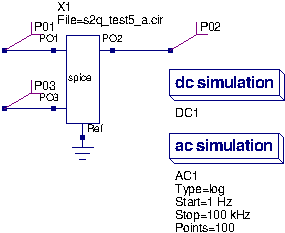
\includegraphics[width=0.6\linewidth]{s2q_5_a_sch} 
  \caption{April 17: Inductor DC and AC test schematic for file s2q\_5\_a.cir}
  \label{fig:s2q_5_a_sch}
\end{figure} 

\begin{figure}
  \centering
  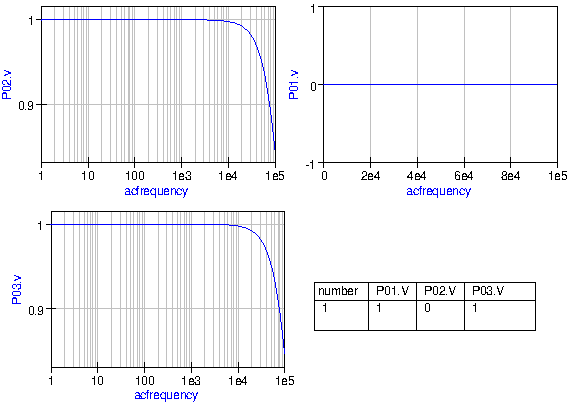
\includegraphics[width=0.7\linewidth]{s2q_5_a_dpl} 
  \caption{April 17: Inductor DC and AC tests results for file s2q\_5\_a.cir}
  \label{fig:s2q_5_a_dpl}
\end{figure} 

\begin{figure}
\begin{lstlisting}[
 language=Clean, 
 basicstyle=\footnotesize]
# Qucs 0.0.12  /media/hda2/S2Q_test5_prj/test_s2q_5_a.sch

.Def:s2q_test5_a_cir _netPO1 _netPO2 _netPO3 _ref
  .Def:S2Q_TEST5_A _ref _netPO1 _netPO2 _netPO3
  Vac:V3 _net3 _cnet1 U="1V"
  Vac:V2 _net2 _cnet0 U="1V"
  Vdc:V1 _net1 _ref U="1V"
  L:L1 _net1 _netPO1 L="1mH"
  R:R1 _netPO1 _ref R="1k"
  Vdc:V2 _cnet0 _ref U="0"
  L:L2 _net2 _netPO2 L="1mH"
  R:R2 _netPO2 _ref R="1k"
  Vdc:V3 _cnet1 _ref U="1V"
  L:L3 _net3 _netPO3 L="1mH"
  R:R3 _netPO3 _ref R="1k"
  .Def:End
  Sub:X1 _ref _netPO1 _netPO2 _netPO3 Type="S2Q_TEST5_A"
.Def:End


Sub:X1 P01 P02 P03 gnd Type="s2q_test5_a_cir"
.AC:AC1 Type="log" Start="1 Hz" Stop="100 kHz" Points="100" Noise="no"
.DC:DC1 Temp="26.85" reltol="0.001" abstol="1 pA" vntol="1 uV" 
saveOPs="no" MaxIter="150" saveAll="no" convHelper="none" Solver="CroutLU"

\end{lstlisting}
 \caption{April 17: s2q\_5\_a Qucs netlist}
  \label{fig:s2q_5_a_qucs}
\end{figure} 




\begin{figure}
  \centering
  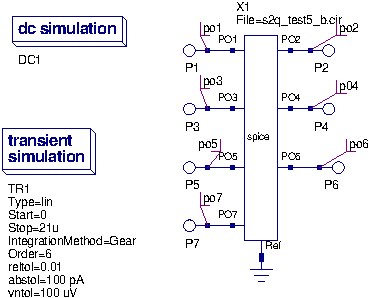
\includegraphics[width=0.6\linewidth]{s2q_5_b_sch} 
  \caption{April 17: Inductor DC and transient test schematic for file s2q\_5\_b.cir}
  \label{fig:s2q_5_b_sch}
\end{figure} 

\begin{figure}
  \centering
  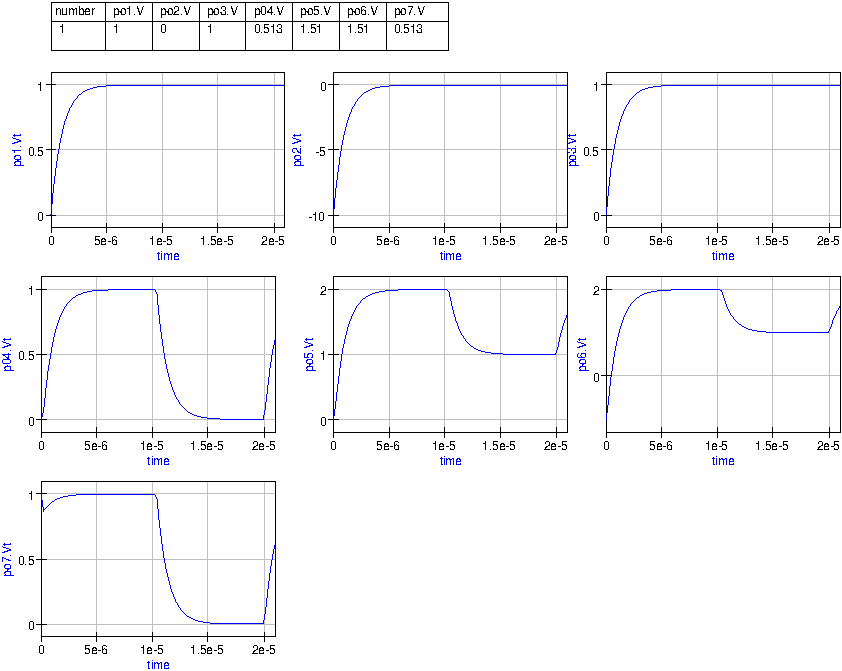
\includegraphics[width=1.0\linewidth]{s2q_5_b_dpl} 
  \caption{April 17: Inductor DC and transient tests results for file s2q\_5\_b.cir}
  \label{fig:s2q_5_b_dpl}
\end{figure} 

\begin{figure}
\begin{lstlisting}[
 language=Clean, 
 basicstyle=\footnotesize]
# Qucs 0.0.12  /media/hda2/S2Q_test5_prj/test_s2q_5_b.sch

.Def:s2q_test5_b_cir _netPO1 _netPO2 _netPO3 _netPO4 _netPO5 _netPO6
 _netPO7 _ref
  .Def:S2Q_TEST5_A _ref _netPO1 _netPO2 _netPO3 _netPO4 _netPO5 _netPO6 
_netPO7
  Vrect:V7 _net7 _cnet3 U="1" Td="0.1u" Tr="0.1u" Tf="0.1u" TH="1.02e-05" 
TL="9.7e-06"
  Vrect:V6 _net6 _cnet2 U="1" Td="0.1u" Tr="0.1u" Tf="0.1u" TH="1.02e-05" 
TL="9.7e-06"
  Vrect:V5 _net5 _cnet1 U="1" Td="0.1u" Tr="0.1u" Tf="0.1u" TH="1.02e-05" 
TL="9.7e-06"
  Vrect:V4 _net4 _cnet0 U="1" Td="0.1u" Tr="0.1u" Tf="0.1u" TH="1.02e-05" 
TL="9.7e-06"
  Vdc:V1 _net1 _ref U="1V"
  L:L1 _net1 _netPO1 L="1mH" I="0mA"
  R:R1 _netPO1 _ref R="1k"
  Vdc:V2 _net2 _ref U="0V"
  L:L2 _net2 _netPO2 L="1mH" I="-10mA"
  R:R2 _netPO2 _ref R="1k"
  Vdc:V3 _net3 _ref U="1V"
  L:L3 _net3 _netPO3 L="1mH" I="0mA"
  R:R3 _netPO3 _ref R="1k"
  Vdc:V4 _cnet0 _ref U="0"
  L:L4 _net4 _netPO4 L="1mH" I="0mA"
  R:R4 _netPO4 _ref R="1k"
  Vdc:V5 _cnet1 _ref U="1"
  L:L5 _net5 _netPO5 L="1mH" I="0mA"
  R:R5 _netPO5 _ref R="1k"
  Vdc:V6 _cnet2 _ref U="1"
  L:L6 _net6 _netPO6 L="1mH" I="-1mA"
  R:R6 _netPO6 _ref R="1k"
  Vdc:V7 _cnet3 _ref U="0"
  L:L7 _net7 _netPO7 L="1mH" I="1mA"
  R:R7 _netPO7 _ref R="1k"
  .Def:End
  Sub:X1 _ref _netPO1 _netPO2 _netPO3 _netPO4 _netPO5 _netPO6 _netPO7 
Type="S2Q_TEST5_A"
.Def:End

.DC:DC1 Temp="26.85" reltol="0.001" abstol="1 pA" vntol="1 uV" saveOPs="no"
 MaxIter="150" saveAll="no" convHelper="none" Solver="CroutLU"
.TR:TR1 Type="lin" Start="0" Stop="21u" Points="100" IntegrationMethod="Gear" 
Order="6" InitialStep="1 ns" MinStep="1e-16" MaxIter="150" reltol="0.01" 
abstol="100 pA" vntol="100 uV" Temp="26.85" LTEreltol="1e-3" 
LTEabstol="1e-6" LTEfactor="1" Solver="CroutLU" relaxTSR="no" 
initialDC="yes" MaxStep="0"
Sub:X1 po1 po2 po3 p04 po5 po6 po7 gnd Type="s2q_test5_b_cir"

\end{lstlisting}
 \caption{April 17: s2q\_5\_b Qucs netlist}
  \label{fig:s2q_5_b_qucs}
\end{figure} 

\begin{figure}
  \centering
  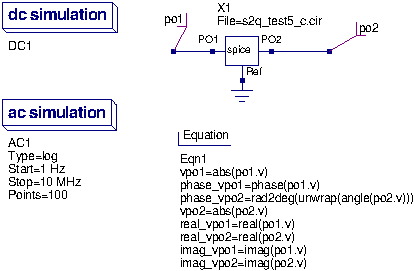
\includegraphics[width=0.6\linewidth]{s2q_5_c_sch} 
  \caption{April 17: Mutual inductance AC test schematic for file s2q\_5\_c.cir}
  \label{fig:s2q_5_c_sch}
\end{figure} 

\begin{figure}
  \centering
  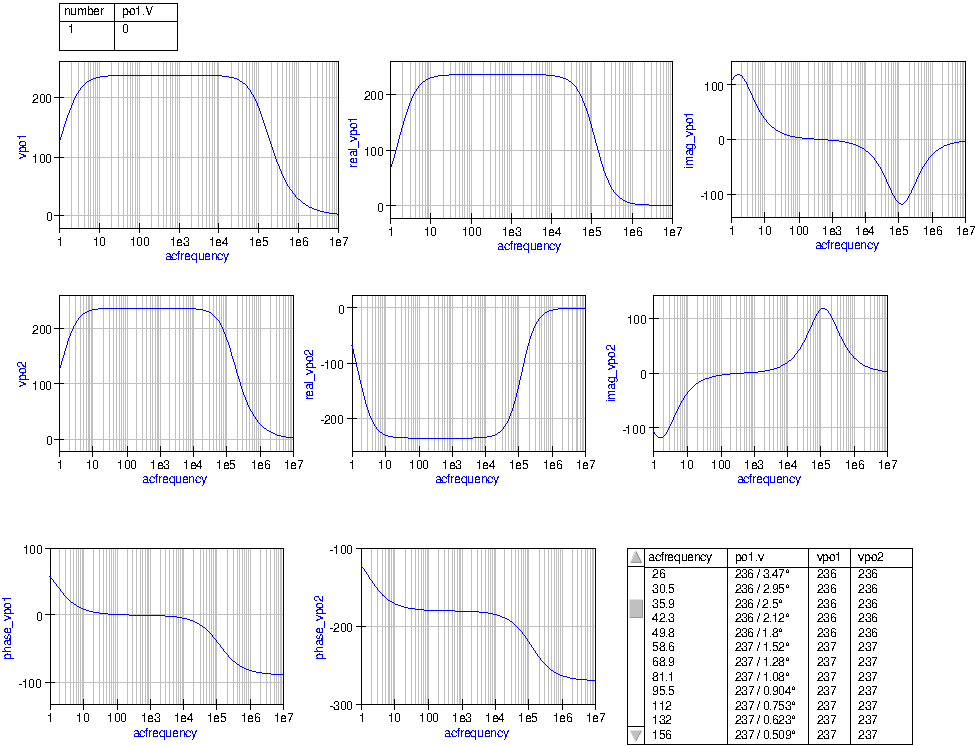
\includegraphics[width=1.0\linewidth]{s2q_5_c_dpl} 
  \caption{April 17: Mutual inductance tests results for file s2q\_5\_c.cir}
  \label{fig:s2q_5_c_dpl}
\end{figure} 

\begin{figure}
\begin{lstlisting}[
 language=Clean, 
 basicstyle=\footnotesize]
# Qucs 0.0.12  /media/hda2/S2Q_test5_prj/test_s2q_5_c.sch

.Def:s2q_test5_c_cir _netPO1 _netPO2 _ref
  .Def:S2Q_TEST5_C _ref _netPO1 _netPO2
  L:K231 _cnet3 _ref L="0.0999"
  L:K23 _cnet1 _ref L="0.0999"
  Vac:V1 _net1 _cnet0 U="240"
  Vdc:V1 _cnet0 _ref U="0"
  R:R1 _net1 _net2 R="1Ohm"
  L:L1 _net2 _cnet1 L="0.0001"
  L:L2 _net3 _cnet2 L="0.0001"
  Tr:K23 _cnet1 _cnet2 _ref _ref T="1"
  R:R2 _net3 _netPO1 R="1Ohm"
  R:RL _netPO1 _ref R="150"
  R:R11 _net1 _net21 R="1Ohm"
  L:L11 _net21 _cnet3 L="0.0001"
  L:L21 _ref _cnet4 L="0.0001"
  Tr:K231 _cnet3 _cnet4 _net31 _ref T="1"
  R:R21 _net31 _netPO2 R="1Ohm"
  R:RL1 _netPO2 _ref R="150"
  .Def:End
  Sub:X1 _ref _netPO1 _netPO2 Type="S2Q_TEST5_C"
.Def:End


.DC:DC1 Temp="26.85" reltol="0.001" abstol="1 pA" vntol="1 
uV" saveOPs="no" MaxIter="150" saveAll="no" convHelper="none" Solver="CroutLU"
.AC:AC1 Type="log" Start="1 Hz" Stop="10 MHz" Points="100" Noise="no"
Sub:X1 po1 po2 gnd Type="s2q_test5_c_cir"
Eqn:Eqn1 vpo1="abs(po1.v)" phase_vpo1="phase(po1.v)" 
phase_vpo2="rad2deg(unwrap(angle(po2.v)))" vpo2="abs(po2.v)" 
real_vpo1="real(po1.v)" real_vpo2="real(po2.v)" imag_vpo1="imag(po1.v)" 
imag_vpo2="imag(po2.v)" Export="yes"

\end{lstlisting}
 \caption{April 17: s2q\_5\_c Qucs netlist}
  \label{fig:s2q_5_c_qucs}
\end{figure} 

\begin{figure}
  \centering
  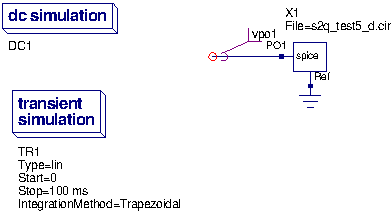
\includegraphics[width=0.6\linewidth]{s2q_5_d_sch} 
  \caption{April 17: Mutual inductance transient test schematic for file s2q\_5\_d.cir}
  \label{fig:s2q_5_d_sch}
\end{figure} 

\begin{figure}
  \centering
  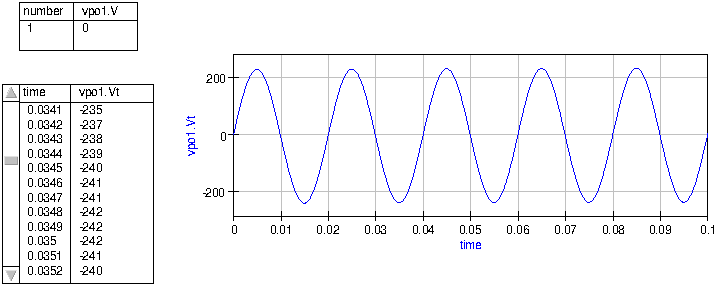
\includegraphics[width=1.0\linewidth]{s2q_5_d_dpl} 
  \caption{April 17: Mutual inductance transient tests results for file s2q\_5\_d.cir}
  \label{fig:s2q_5_d_dpl}
\end{figure} 

\begin{figure}
\begin{lstlisting}[
 language=Clean, 
 basicstyle=\footnotesize]
# Qucs 0.0.12  /media/hda2/S2Q_test5_prj/test_s2q_d.sch

.Def:s2q_test5_d_cir _netPO1 _ref
  .Def:S2Q_TEST5_C _ref _netPO1
  L:K23 _cnet1 _ref L="0.0999"
  Vac:V1 _net1 _cnet0 U="240" f="50" Phase="-0" Theta="0"
  Vdc:V1 _cnet0 _ref U="0"
  R:R1 _net1 _net2 R="1Ohm"
  L:L1 _net2 _cnet1 L="0.0001"
  L:L2 _net3 _cnet2 L="0.0001"
  Tr:K23 _cnet1 _cnet2 _ref _ref T="1"
  R:R2 _net3 _netPO1 R="1Ohm"
  R:RL _netPO1 _ref R="150"
  .Def:End
  Sub:X1 _ref _netPO1 Type="S2Q_TEST5_C"
.Def:End


Sub:X1 vpo1 gnd Type="s2q_test5_d_cir"
.DC:DC1 Temp="26.85" reltol="0.001" abstol="1 pA" 
vntol="1 uV" saveOPs="no" MaxIter="150" saveAll="no" 
convHelper="none" Solver="CroutLU"
.TR:TR1 Type="lin" Start="0" Stop="100 ms" Points="1000" 
IntegrationMethod="Trapezoidal" Order="2" InitialStep="1 ns" 
MinStep="1e-16" MaxIter="150" reltol="0.001" abstol="1 pA" 
vntol="1 uV" Temp="26.85" LTEreltol="1e-3" LTEabstol="1e-6" 
LTEfactor="1" Solver="CroutLU" relaxTSR="no" initialDC="yes" MaxStep="0"

\end{lstlisting}

 \caption{April 17: s2q\_5\_d Qucs netlist}
  \label{fig:s2q_5_d_qucs}
\end{figure} 



\begin{figure}
  \centering
  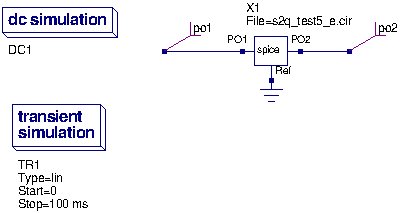
\includegraphics[width=0.8\linewidth]{s2q_5_e_sch} 
  \caption{April 17: Mutual inductance transient test schematic for file s2q\_5\_e.cir}
  \label{fig:s2q_5_e_sch}
\end{figure} 

\begin{figure}
  \centering
  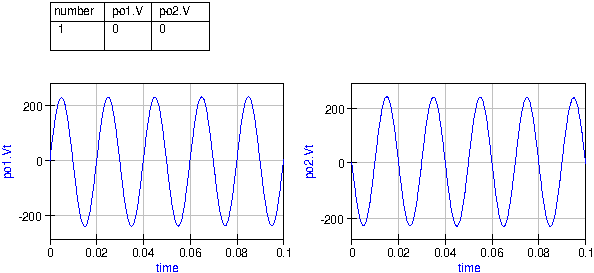
\includegraphics[width=1.0\linewidth]{s2q_5_e_dpl} 
  \caption{April 17: Mutual inductance transient tests results for file s2q\_5\_e.cir}
  \label{fig:s2q_5_e_dpl}
\end{figure} 

\begin{figure}
\begin{lstlisting}[
 language=Clean, 
 basicstyle=\footnotesize]
# Qucs 0.0.12  /media/hda2/S2Q_test5_prj/test_s2q_5_e.sch

.Def:s2q_test5_e_cir _netPO1 _netPO2 _ref
  .Def:S2Q_TEST5_C _ref _netPO1 _netPO2
  Vac:V1 _net1 _cnet0 U="240" f="50" Phase="-0" Theta="0"
  Vdc:V1 _cnet0 _ref U="0"
  R:R1 _net1 _net2 R="1Ohm"
  MUT2:K12K13K23 _net2 _ref _net4 _ref _net3 _ref L1="0.1" L2="0.1"
  L3="0.1" k12="0.999" k13="0.999" k23="0.999"
  R:R2 _net3 _netPO1 R="1Ohm"
  R:RL1 _netPO1 _ref R="150"
  R:R3 _net4 _netPO2 R="1Ohm"
  R:RL2 _netPO2 _ref R="150"
  .Def:End
  Sub:X1 _ref _netPO1 _netPO2 Type="S2Q_TEST5_C"
.Def:End


Sub:X1 po1 po2 gnd Type="s2q_test5_e_cir"
.DC:DC1 Temp="26.85" reltol="0.001" abstol="1 pA" vntol="1 uV" saveOPs="no" 
MaxIter="150" saveAll="no" convHelper="none" Solver="CroutLU"
.TR:TR1 Type="lin" Start="0" Stop="100 ms" Points="1000" 
IntegrationMethod="Trapezoidal" Order="2" InitialStep="1 ns" 
MinStep="1e-16" MaxIter="150" reltol="0.001" abstol="1 pA" vntol="1 uV" 
Temp="26.85" LTEreltol="1e-3" LTEabstol="1e-6" LTEfactor="1" 
Solver="CroutLU" relaxTSR="no" initialDC="yes" MaxStep="0"

\end{lstlisting}

 \caption{April 17: s2q\_5\_e Qucs netlist}
  \label{fig:s2q_5_e_qucs}
\end{figure} 



